\section*{Title I School Funding Allocation}

\subsection{Allocation Problem}
The \emph{Title I of the Elementary and Secondary Education Act of
1965} \cite{Sonnenberg:16} distributes funds through its basic, concentration, and target grants which account for \$6.2B, \$1.3B, and \$4.2B of allocations, respectively. The federal allotment is divided among nearly 17000 qualifying school
districts in proportion to the count $x_i$ of children aged 5 to 17
who live in necessitous families in district $i$. Each grant is specified by a set of thresholds that determines which districts are eligible for that particular grant. We refer to \cite{Sonnenberg:16} which discusses the specifics of each grant, which we describe briefly here.

The basic allocation grant is formalized by:
\newcommand{\tfa}{P^F}
\newcommand{\rev}[1]{{\color{purple}{#1}}}
\newcommand{\add}[1]{{\color{darkgreen}{#1}}}
\newcommand*{\defeq}{\stackrel{\text{def}}{=}}
\def\aux{\mathrm{aux}}

\begin{align}
	\label{eq:allotment}%\tag{\text{$P_1$}}
	\tfa_i(\bm{x}) \defeq \left(
	\frac{x_i \cdot a_i}{\sum_{i \in [n] }x_i \cdot a_i}\right) \cdot F_{B}
\end{align}
where $\bm{x} = (x_i)_{i\in[n]}$ is the vector of all eligible districts counts
and $a_i$ is a weight factor reflecting students expenditures (defined as the adjusted state per-pupil expenditure). $F_{B}$ is the total basic Title I appropriation for the fiscal year. Finally, each funding grant is subject to different thresholds which define eligibility criteria for each district. This criteria is described in Table 1. The targeted grant is further weighted by population, as outlined in Section A of \cite{Sonnenberg:16}.

\begin{table}[t!]
	\centering
	\caption{Description of the thresholds that construct the eligibility criteria for each grant.}
	\begin{tabular}{lrr}
		\toprule
		Grant Type        & Eligibility Criteria            & Thresholds \\
		\midrule
		Basic Grant         & Population of eligible students & $>10$      \\
		& Proportion of eligible students & $>0.02$    \\
		Concentration Grant & District population             & $>6500$    \\
		& Proportion of eligible students & $>0.15$    \\
		Targeted Grant      & Population of eligible students & $>10$      \\
		& Proportion of eligible students & $>0.05$    \\
		\bottomrule
	\end{tabular}
	\medskip
	\raggedright
\end{table}

\subsection{Privacy Budget}
The Disclosure Avoidance System for the US Census Bureau defines a global rho that is distributed hierarchically.
The global privacy-loss budget for 2020 was defined as $\rho = 2.56$. The DAS suggests the use of this bound to conver
the $\rho$-based privacy-loss budgets to the $(\epsilon, \delta)$ equivalents.
$\epsilon = \rho + 2 * \sqrt{-\rho * \log_e{\delta}}$ where we define $\delta=10e-10$. In a 1-year estimate of the ACS,
there are $1426$ different "Detailed tables" available from the US Census Bureau. The rho allocation for the national,
state, and county level geographic hierarchies are $\frac{104}{4099}$, $\frac{1440}{4099}$, and $\frac{447}{4099}$
respectively. Assuming that the county level privacy-loss budget is split equally across these tables,
each field would have $\rho = 2.56 \cdot \frac{447}{4099} \cdot \frac{1}{1426} = 0.0001957 $ at the county level,
$\rho = 0.00063$ at the state level, and $\rho = 0.0000455$ at the national level.

We consider applying the Gaussian mechanism to satisfy differential privacy on children population estimate data along
with a hierarchical constraint that ensures that the sum of the noisy population estimate of sub-hierarchies are
consistent with their parent. For example, the sum of Title I-eligible children in the county-level subdivisions
of Illinois should be consistent with the noisy estimate of Title I-eligible children at the state level. We experiment
with three privacy budgets $\rho =  2.65$ and $\rho = 1.0$ and $\rho = 0.1$ to release privately the schools' population. These
private counts are used to determine amount of money each school district should receive using the allocation mechanisms
described above for the basic, concentration, and target grants. The statistical bias in Definition \ref{def:bias} here
represents the gain/loss in USD a school can have under the privacy preserving mechanism. \ref{fig:misalloc_total}
summarizes our findings of the bias as a function of district size for all $13,190$ districts. We observe that
misallocations are most pronounced at thresholds for each grant, and substantially impact smaller school districts more
than larger ones.

\begin{figure*}[h]
	\centering
	\begin{minipage}[b]{0.45\linewidth}
		\centering
		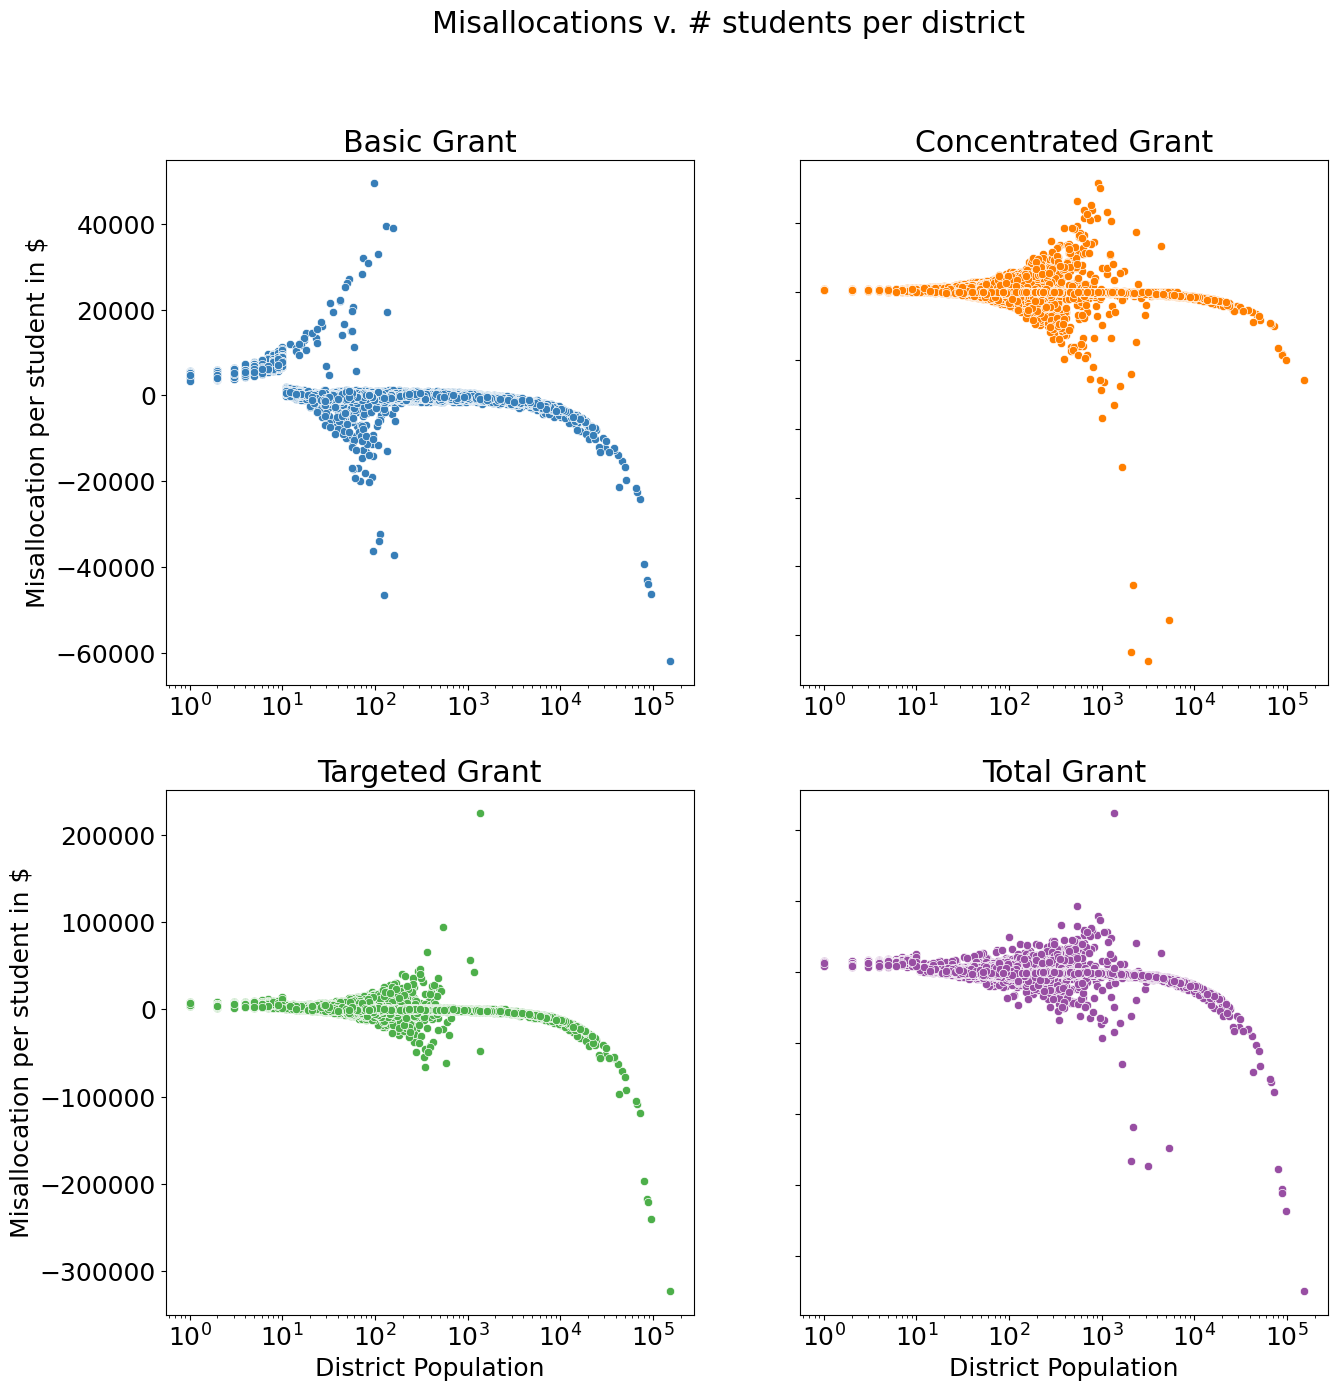
\includegraphics[width=\linewidth]{images/all_grant_errors_total}
		\caption{Misallocations in USD compared to district size}
		\label{fig:misalloc_total}
	\end{minipage}
	\hfill
	\begin{minipage}[b]{0.45\linewidth}
		\centering
		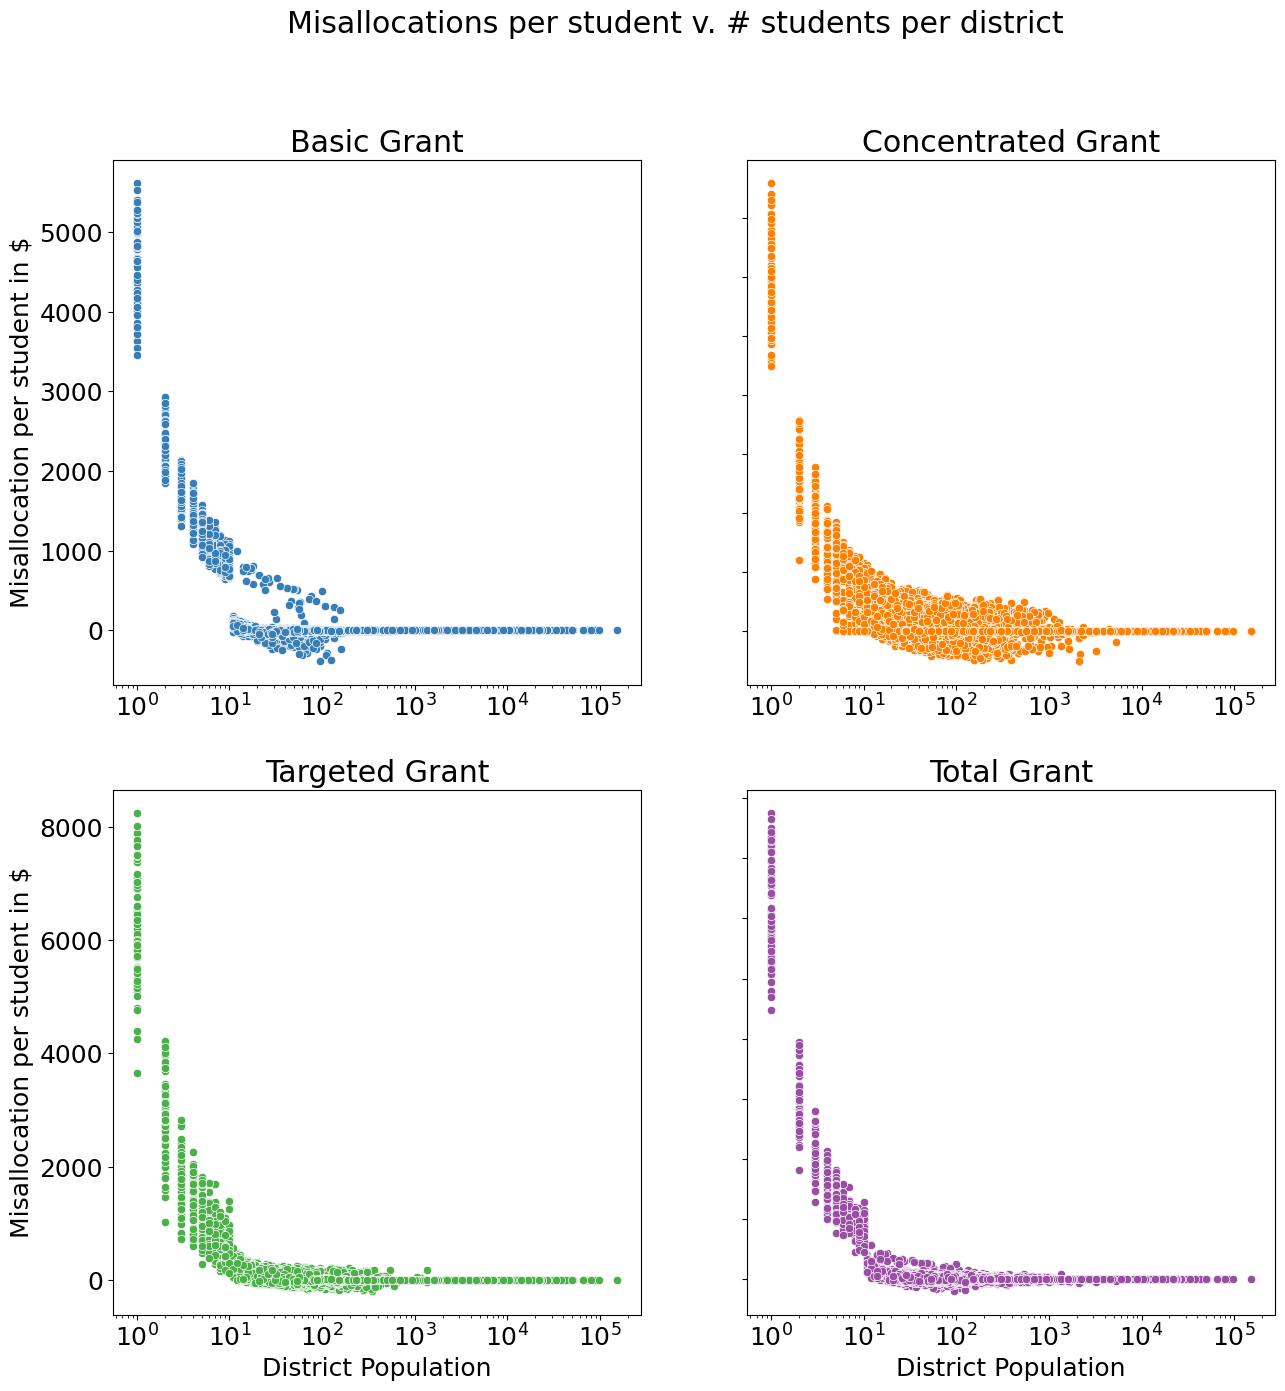
\includegraphics[width=\linewidth]{images/all_grant_errors_per_capita}
		\caption{Misallocations in USD per student compared to district size}
		\label{fig:misalloc_per_student}
	\end{minipage}
	\caption{We apply differential privacy with a privacy budget of $\rho=2.65$ to the population and eligible
	population counts of each district. We then plot the Title I misallocations for each district in the US for the
	basic, concentrated, and targeted grants, calculated using the allocation formulas outlined in \cite{Sonnenberg:16}.
	We observe that while large districts are more likely to receive larger misallocations, smaller districts are more
	likely to receive larger misallocations per student. We attribute these results to the complex interaction
	between differential privacy and the thresholds in the allocation formulas.}
	\label{fig:misalloc_comparison}
\end{figure*}


\begin{figure}[!ht]
	\centering
	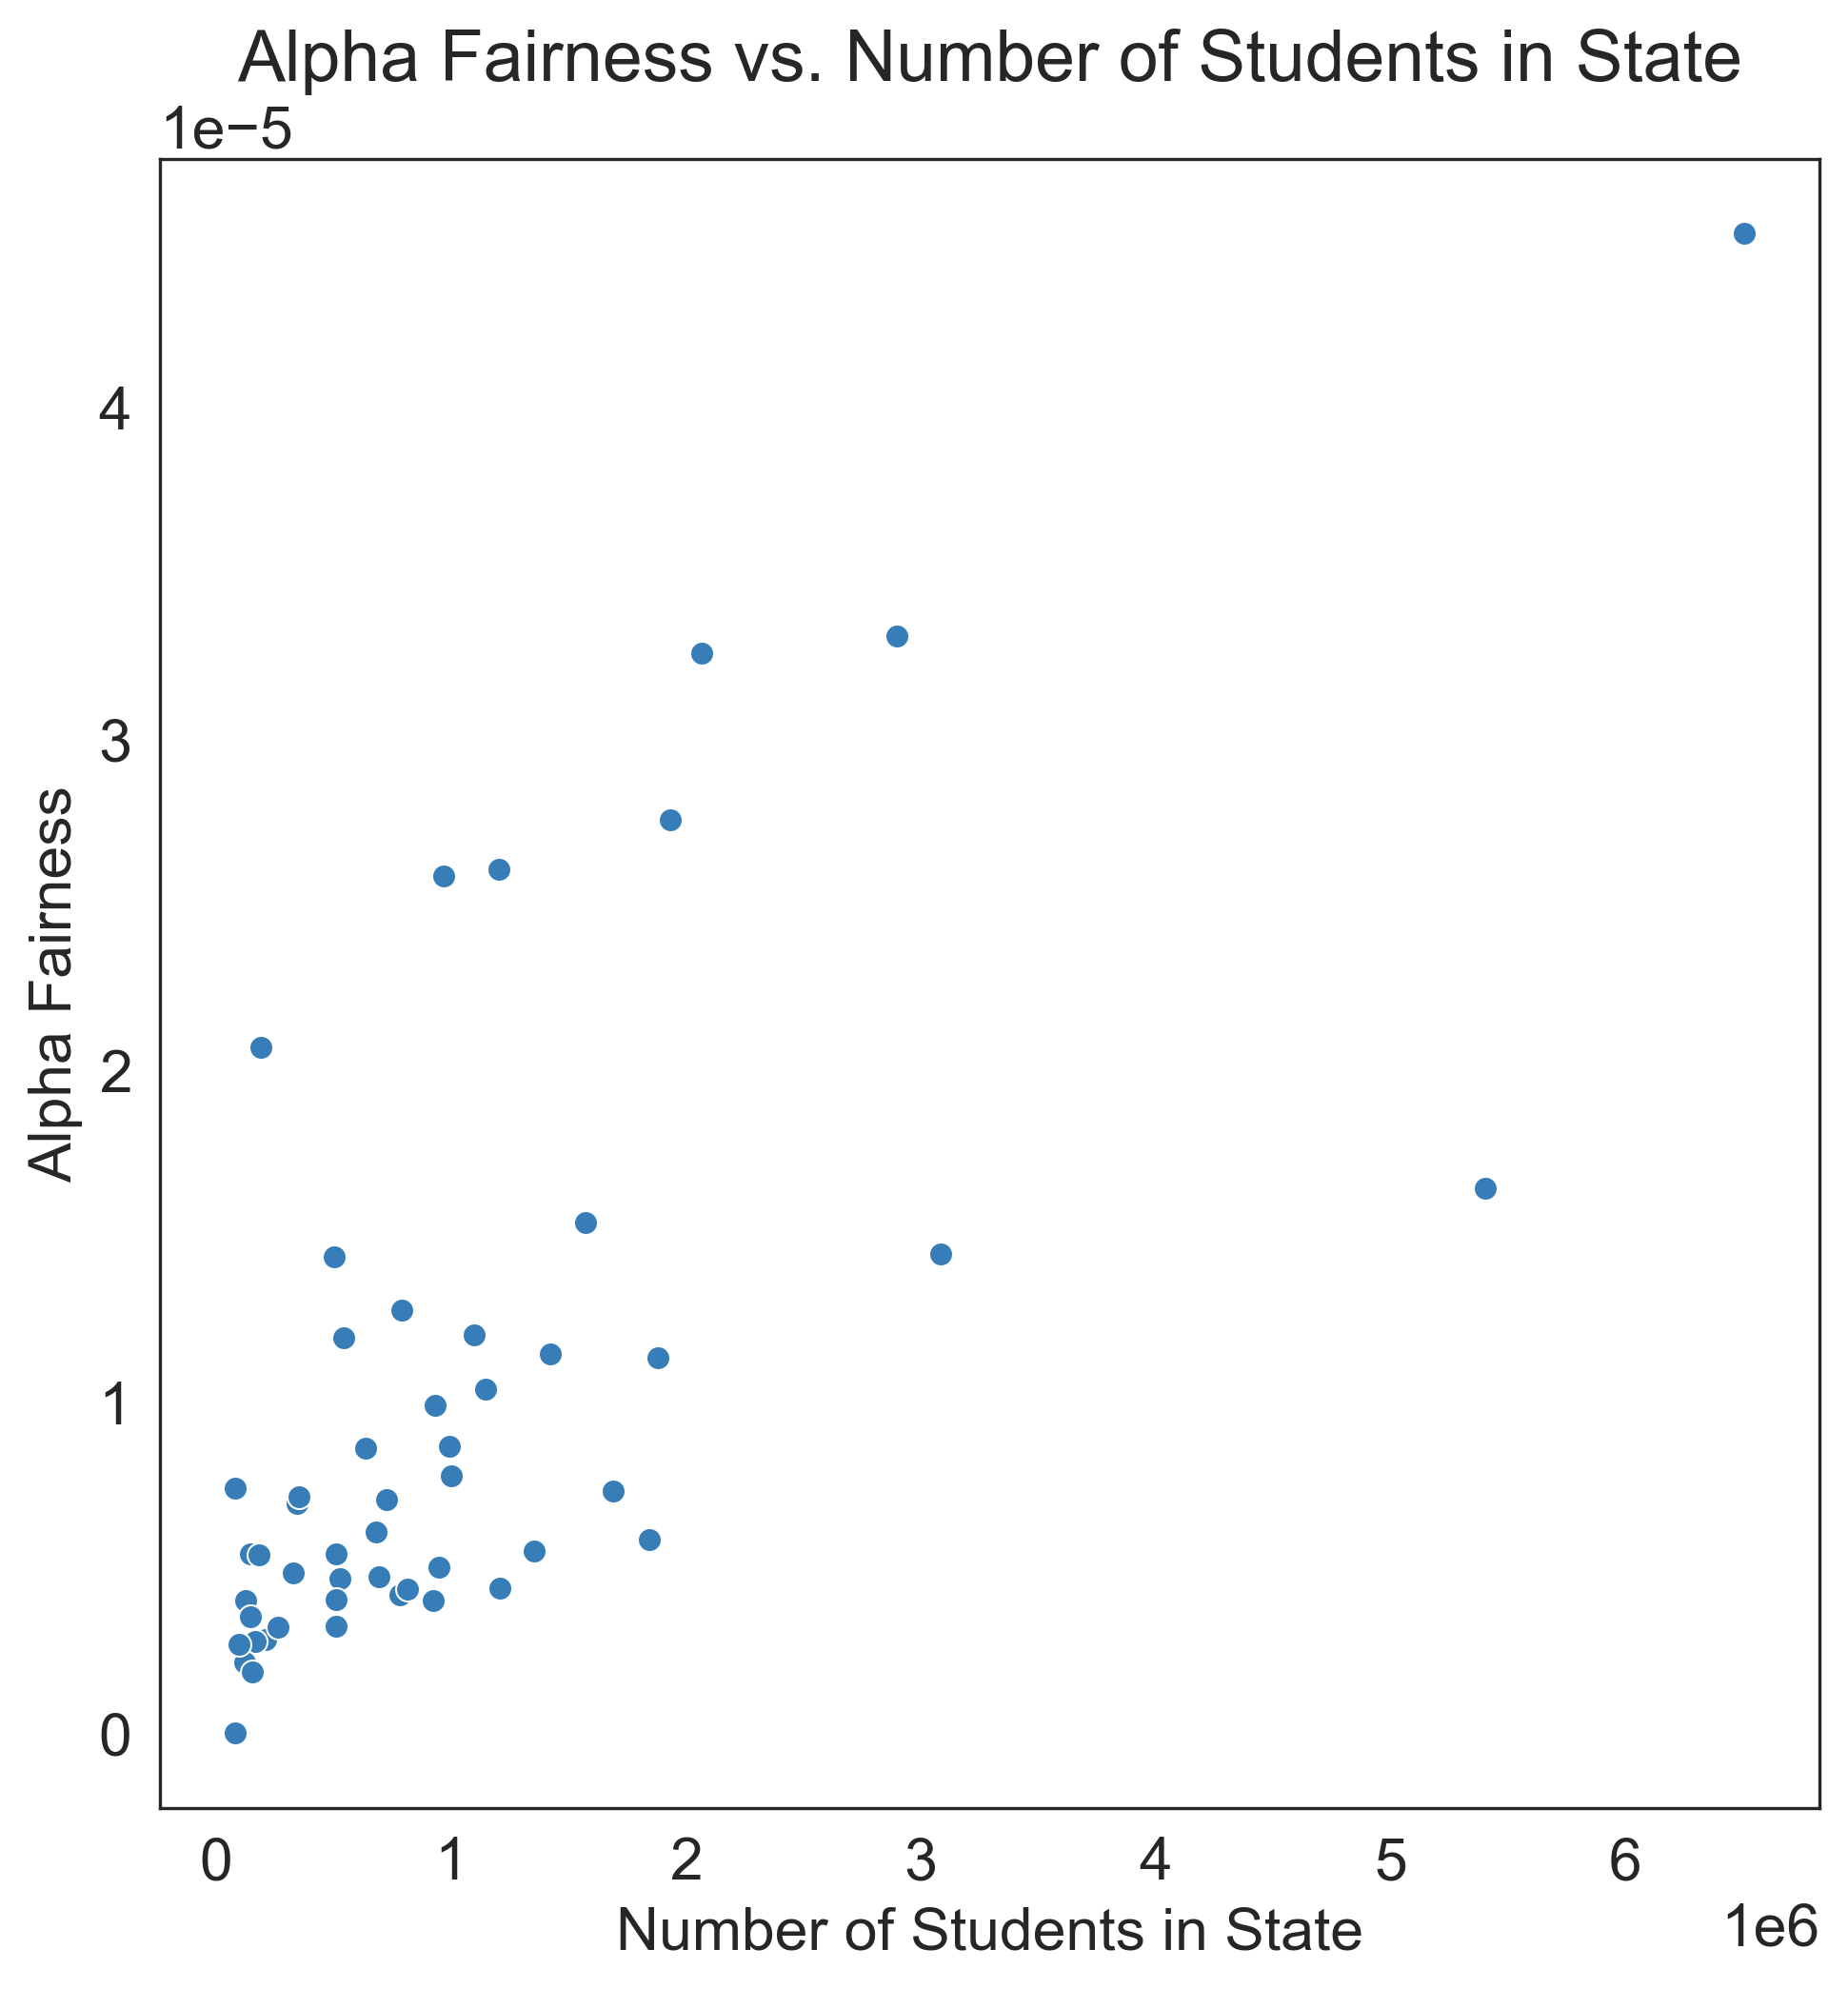
\includegraphics[width=0.6\linewidth]{images/af_vs_num_students_per_state}
	\caption{Correlation between number of students per state and alpha fairness at $\rho=2.65$}
	\label{fig:corr_fair_num_students}
\end{figure}


\begin{figure*}[h]
	\centering
	\begin{minipage}[b]{0.45\linewidth}
		\centering
		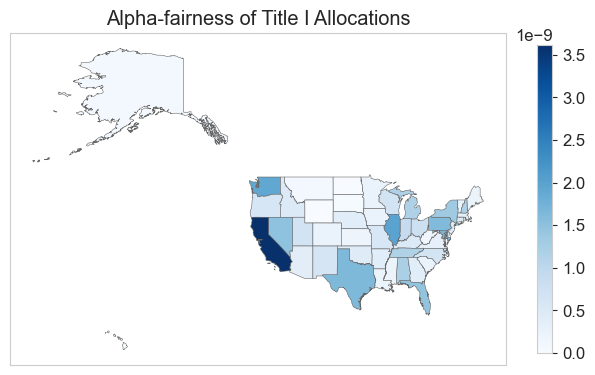
\includegraphics[width=\linewidth]{images/af_by_state.png}
		\caption{Level of $\alpha$ fairness per state under Baseline mechanism (BL) at $\rho = 2.56$}
		\label{fig:state_alpha}
	\end{minipage}
	\hfill
	\begin{minipage}[b]{0.45\linewidth}
		\centering
		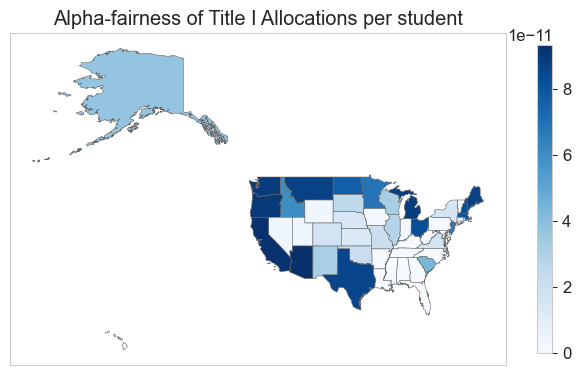
\includegraphics[width=\linewidth]{images/af_by_student.png}
		\caption{Level of $\alpha$ fairness per student under Baseline mechanism (BL) at $\rho = 2.56$}
		\label{fig:student_alpha}
	\end{minipage}
	\caption{Fairness comparison}
	\label{fig:fairness_comparison}
\end{figure*}



It can be seen from Figure \ref{fig:misalloc_total} that schools of low population receive far more money than they actually need
as a consequence of the bias in the allocation mechanism, while larger districts may actually receive less funding. This figure made a clear evidence on the disparate impact of the privacy preserving mechanism in practice.


\subsection*{Analysis}
In order to probe the effects of applying differential privacy to the Title I Allocation problem, we simulate
applying DP and recomputing grants for each district based on the distribution formula described by \cite{Sonnenberg
:16}. We compute 100K trials of samples to construct figures \ref{fig:misalloc_total} and the rest of our analysis.
We attribute the complex funding misallocation outcomes to the interaction of the several thresholds that consistute
each grant.

An in-depth analysis of the allocation of Title I education funds in districts requires an examination of both total
misallocations and misallocations per student. The consideration of these two perspectives is crucial for
understanding the impact of differential privacy on the distribution of funds and its implications for educational
equity.

Total misallocations offer a comprehensive overview by capturing the absolute magnitude of funding disparities across
states. By assessing the overall amount of misallocated funds, we can identify states that are disproportionately
affected. Such significant total misallocations can result in substantial disparities in educational resources,
thereby hindering the ability of disadvantaged districts to provide quality education. The findings from \ref{fig:misalloc_total},
which displays the data on total misallocations for each type of grant (basic, concentration, and targeted
), reaffirm this observation.

However, evaluating misallocations per student provides a more nuanced understanding of the fairness of funding
distribution. This perspective allows us to account for the relative impact on individual students within each state
. Misallocations per student highlight the distributional challenges faced by specific states and reveal the extent
to which educational inequalities are exacerbated. The data presented in Figure \ref{fig:misalloc_per_student}, whic
depicts misallocations per student, demonstrate that smaller districts tend to gain a substantial amount of funds
due to the application of differential privacy. In contrast, larger districts experience significant misallocations
without necessarily facing the same level of negative impact on a per-student basis.

It is important to recognize the specific implications of misallocations in different contexts. When funds are
misallocated in total, certain types of funding, such as specialized educational programs, additional resources, or
support services for at-risk students, may be inadequately supported. This can perpetuate existing disparities and
hinder efforts to address educational inequities, particularly in states with a higher population of disadvantaged
students. On the other hand, misallocations per student shed light on the deprivation of financial support
individual students require to succeed academically. This impacts the availability of crucial resources, including
instructional materials, qualified teachers, technology, and extracurricular activities, thereby impeding
educational progress and perpetuating systemic inequalities.

The correlation between a state's student population and the alpha fairness, as shown in
\ref{fig:corr_fair_num_students}, further supports the observed disparities. The positive Pearson correlation coefficient of
0.76 indicates that states with larger populations of students tend to have higher levels of alpha fairness,
indicating a greater degree of inequitable fund allocation.

Thus, the analysis of both total misallocations and misallocations per student provides a comprehensive understanding
of the impact of differential privacy on the allocation of Title I education funds. This dual perspective enables
policymakers to identify states disproportionately affected in terms of both the absolute amount of misallocated
funds and the relative impact on individual students. By gaining insights into the specific challenges faced by
different states, policymakers can devise targeted strategies to ensure a fair and equitable distribution of
education funds, taking into account the disparities arising from both large total misallocations in large districts
and smaller misallocations per student in small districts (Figure \ref{fig:misalloc_comparison}).
